\chapter{Implementation}



\section{ECMAScript and JavaScript}
ECMAScript \footnote{http://www.ecmascript.org/} is a standardized scripting language widely used in website development. Latest approved edition of ECMAScript is \textit{ECMAScript 5.1}, which is implemented in most major web browsers, and its implementations in web browsers are commonly called JavaScript \footnote{https://developer.mozilla.org/en/docs/Web/JavaScript}\footnote{https://msdn.microsoft.com/cs-cz/library/d1et7k7c(v=vs.94).aspx}. 

JavaScript is a dynamic programming language \footnote{http://en.wikipedia.org/wiki/Dynamic\_programming\_language}, which combines multiple aspects of imperative, functional, and object-oriented programming.

Functions are so called first-class citizens. This means they can be stored in variables, passed as function parameters, returned as results of functions, and included in data structures.

JavaScript doesn't provide any means of static type checking. All types are created during runtime and they are also checked only during runtime. The lack of static type checking during compilation might lead to rarely occurring errors and it is important to take this in mind while writing JavaScript code. A good practice is to write documentation comments\footnote{Commonly used syntax in JavaScript projects is JSDoc (http://usejsdoc.org/)}, where the types are stated.

JavaScript is an interpreted language, some implementations also use a Just-In-Time compilation (JIT) \footnote{For example Google V8 engine used in Google Chrome. See https://code.google.com/p/v8/} for better performance.  Another very important aspect of ECMAScript which affects its performance is the absence of direct control over memory usage -- memory is released when it is not needed any more. This mechanism is called \textit{Garbage collection}. As of 2012, all modern browsers use mark-and-sweep garbage-collector \cite{mdn_memmory_management}.

\textit{Object oriented programming} (OOP) \footnote{http://en.wikipedia.org/wiki/Object-oriented\_programming} in JavaScript differs from class-oriented OOP in the way inheritance is implemented. While in class-oriented languages, for example in C++ or C\#, inheritance is achieved by declaring classes of objects. In JavaScript, OOP is implemented through object prototypes. Prototype is just a link to another object, which has another prototype. A prototype chain is created this way. The last object in this chain has a \verb|null| prototype. When trying to access a property of an object, it is searched in its own properties. If it is not found, then it is searched in its prototype's properties and so on until the end of the prototype chain is reached \cite{mdn_prototype_chain}.

\subsection{TypeScript}
\textit{TypeScript} is a typed superset of JavaScript that compiles to plain JavaScript\cite{typescript}. It is an open-source project developed by Microsoft. It is, as its name suggests, a strongly typed programming language compatible with JavaScript.

TypeScript extends capabilities of JavaScript by static type checking at the time of compilation, which helps the programmer to find errors in source code sooner, and speeds up the process of coding. TypeScript also introduces \textit{class} semantics. These classes are transpiled into JavaScript prototypes. TypeScript also includes concepts of interfaces and polymorphism, which makes programs written in TypeScript more understandable to programmers familiar with other object-oriented programming languages like Java, C\# or C++.

TypeScript uses several features of ECMAScript 6, but it is transpiled into ECMAScript 5.1, and therefore does not bring any new functionality. The reason for choosing TypeScript is the clarity of code and more convenient development process for the programmer.



\section{Event driven programming}
The idea behind event driven programming is to break direct references between objects and to communicate with \textit{events} instead of calling object methods directly. The advantage of the this approach is the so called \textit{loose coupling} \cite{loose_coupling} -- features might be added or removed without breaking the core of the application.

Each object handles only it's own task without knowing anything about the other objects it's collaborating with. When an object completes it's task, it publishes the result with a specific event. Objects subscribed for this event are notified and are given the outcomes of the previous task.

This mechanism is sometimes called the \textit{Event Aggregator} design pattern. It is implemented through the \verb{VideoEvents}\footnote{Implementation can be found in \textit{/public/js/app/Helpers/VideoEvents.ts} file} static class, which makes it a simple singleton object. This class provides an interface for registering and triggering callbacks for specified events. Callbacks executed by a triggered event are called asynchronously. It is worth mentioning that web browsers execute all scripts in a single thread.

\begin{lstlisting}
VideoEvents.on(VideoEventType.Message, function(message) {
  console.log("received message:", message);
});

VideoEvents.on(VideoEventType.Message, function(message) {
  console.log("received message backwards:", message.split("").reverse().join(""));
});

VideoEvents.trigger(VideoEventType.Message, "Hello world.");

\end{lstlisting}

The list of all event types can be found in the enclosed API documentation of the \verb|VideoEventType| enumeration.


\section{HTML5}

HTML5 is a term used to refer to modern web technologies. The core is the \textit{HyperText Markup Language}, designed to describe semantics of structured documents \cite{html5}. HTML5 extends the semantics of HTML 4.1 with new HTML tags such as \verb|<header>| or \verb|<footer>|, but also defines a huge set of new APIs, which allow web developers to create much richer websites and web applications. Some of these new technologies are needed by the Vector Screencasts project.

\paragraph{Working with XML documents}
Working with XML data is very similar to working with regular website DOM\footnote{Document Object Model, http://www.w3.org/DOM/} in JavaScript. \verb|Document|\footnote{https://dom.spec.whatwg.org/\#interface-document} interface is used for traversing the XML tree, modifying it or for creating a new one. In HTML5, XML files can be opened using a HTTP GET request via \verb|XMLHttpRequest|\footnote{https://xhr.spec.whatwg.org/} object, which parses the data and returns a \verb|Document| instance in its \verb|responseXML| property, if the document meets specified criteria \cite{xhr}.

\paragraph{WebSockets}
WebSockets allow applications to open bidirectional communication channels with server-side processes \cite{}\footnote{https://html.spec.whatwg.org/multipage/comms.html\#network}. WebSockets are built on top of the \textit{Transmission Control Protocol} (TCP) connection. This means that the delivery of data is reliable and ordered \cite{}\footnote{https://tools.ietf.org/html/rfc6455}.

\paragraph{Web Workers}
JavaScript code of a website normaly runs in a single thread. It is common to run functions asynchronously, for example callback functions and event handlers, but all these functions still run in the same thread. Web Workers are a means of running heavy tasks in background without affecting the user interface. A real OS-level thread is spawn for each \verb|Worker| object instance.

Web Workers have several limitations. They cannot change the DOM and have direct links to objects in the main thread. Web workers receive messages from the parent thread through an \verb|onmessage| event and can send a response via the \verb|postMessage| function. These messages contain serialized JavaScript objects, which cannot contain any references. As a result, concurrency problems are not typically an issue. Web Workers can perform HTTP requests using the \verb|XMLHttpRequest| object, but the content is not parsed, if the target is an XML or HTML file. For more details see the specification of the Worker object\cite{} \footnote{https://html.spec.whatwg.org/multipage/workers.html\#worker}





\subsubsection{Rendering graphics using HTML5}

Displaying text and static visual content is the main purpose of older versions HTML and \textit{Cascade Style Sheets} (CSS). Creating complex polygons or curves would be very hard, involve various tricks \footnote{http://nicolasgallagher.com/pure-css-gui-icons/} or would be even impossible. 

The new HTML specification takes this in mind and brings ways of creating more rich and dynamic content within a web page. There are two technologies that should be taken into account -- \textit{Canvas 2D Context} and \textit{SVG}.

\paragraph{Canvas 2D Context}
The \verb|<canvas>| element provides scripts with a resolution-dependent bitmap canvas, which can be used for rendering graphs, game graphics, or other visual images on the fly \cite{html5_canvas}. 

Using canvas seems appropriate for this project. Canvas could be created with respect to user's resolution and web browser window size. All elements can be scaled to fit this viewport. This will make them look sharp and there will not be any artefacts, noise and blur caused by interpolation used for scaling regular bitmap video content.

When the dimensions of the \verb|<canvas>| element change, the image is scaled, but the output will not be very sharp. Canvas contains a bitmap image, onto which the graphics primitives are drawn. All these primitives must be redrawn by the programmer to achieve smooth scaling.

\paragraph{SVG} @todo










\section{Drawing lines}
Khan Academy videos are known for their consistent and simple style. A person draws on a virtual canvas (evoking a school blackboard) with a brush (or possibly a chalk) of a round shape.

Tutor has a pointing device, typically a computer mouse or a digital stylus, and its position on the canvas is marked with a moving cursor. When the tutor clicks, a dot is marked on canvas in the current position of the cursor. Tutor can produce a line (typically a curve) following this cursor when he presses a mouse button or increases digital stylus pressure while moving the cursor. The curve ends when he releases the button or lowers stylus pressure. The color and size of the dot or line corresponds to current settings. Pressed mouse button corresponds to maximal applied pressure and released mouse button to no pressure.

Rendering at the time of playback gives us the opportunity to adjust the outcome to the environment of the end user. This means that the result can be sharp on every display resolution without the need of having many versions of the same video for each resolution.

\subsection{Dynadraw algorithm}
\label{sec:dynadraw}

Paul Haeberli has created a simple algorithm called \textit{``Dynadraw''} in 1989, which is suitable for calligraphy. Brush is modeled as a physical object with its \textit{mass}, \textit{velocity} and \textit{friction coefficient} \footnote{Dynadraw: http://www.graficaobscura.com/dyna/index.html} \cite{}. Mouse movement is interpreted as a way of exerting force on the brush -- the faster you move the brush, the greater the force applied on the brush is. Acceleration is then calculated according to Newton's second law of motion considering brush's mass and velocity of the brush is derived with respect to the value of friction coefficient. This velocity is then applied and brush is moved. The trace brush should leave behind is then drawn onto the virtual canvas.

The advantage of this algorithm is its simplicity and the possibilities of configuring the brush with different values of mass and friction (the author of the algorithm refers to this constant also as \textit{drag}, which better fits the purpose of slowing down the brush).

Heavier brushes move slower than the light ones, but the path they leave behind is much smoother, as the hand shaking is eliminated by composition of forces in different directions.

Light brushes move faster and are often very close to the cursor during the movement. When the cursor stops abruptly, light brushes with little friction tend to keep moving past the cursor and wrap around it. This produces little curls at the end of lines.

\subsubsection*{Brush movement simulation}

One step of simulation applies force on the brush according to current mouse position and thus moves it in the direction of the cursor. This process of applying force must be done periodically, at the frequency of 60~Hz in ideal case\footnote{HTML5 provides \text{requestAnimationFrame} function, which is intended for animations and which targets 60 frames per second}. Implementation of this simulation is not identical to the original \textit{Dynadraw} algorithm, but all of its key aspects are preserved. Pseudocode ~\ref{alg:one-step} describes the algorithm used in this thesis.

The main difference between the original implementation and the one used in Vector Screencast project is brush width calculation. The original algorithm calculates the width of the line in a specific point by measuring its velocity -- the faster the brush is moving, the thinner the drawn line is. This width dynamics gave the algorithm its name.

In our implementation, this effect is preserved, but it is much more subtle. Brush dynamics relies mainly on the pressure of a digital stylus on a graphics tablet. Since the exact value of pressure in the point of current brush's location is not always known, the value is linearly interpolated between the value of pressure in the previous position of the brush and the value of pressure in the current mouse position according to the distance from each of these points.

As this simulation is not deterministic, this process cannot be reconstructed afterwards. When the video is being played, only the precomputed values of path segments must be used. The precise value of pressure is therefore irrelevant for later playback of the screencast and does not have to be stored. The advantage of storing this values is the possibility of reconstructing the process of recording later and rendering the lines again. Even a different algorithm might be used in this case.

\begin{pseudocode}
  \begin{algorithmic}

  	\Function{OneStep}{$M$, $\Delta t$} \Comment $M$ - mouse position, $\Delta t$ - elapsed time
      \If {$M \neq \emptyset$}
	      \State $brushMoved \gets \Call{apply}{\vec{M}, \Delta t} $
          \If {$brushMoved = true$}
              \State \Call{DrawSegment}{}
          \EndIf
      \EndIf
 	\EndFunction

	\Function{apply}{$M, \Delta t$}
      \State $ \vec{F} \gets M - P $\Comment $P$ - current position of the brush
      \State $ \vec{a} = \frac{\vec{F}}{m} $\Comment $m$ - mass of the brush

      \If{$ \norm{\vec{a}} \le C_a $} \Comment $C_a$ - minimum acceleration constant
	      \State \Return false;    
       \EndIf
      
      \State $\vec{v} \gets \vec{v} + \vec{a}$

      \If {$ \norm{\vec{v}} > C_v$} \Comment $C_v$ - minimum velocity constant
          \State $ P \gets P + \mu\Delta t\vec{v} $\Comment $\mu$ - coefficient of friction
		  \State \Return true
      \EndIf
      \State \Return false
  	\EndFunction
  \end{algorithmic}
\caption{One step of brush movement simulation}
\label{alg:one-step}
\end{pseudocode}

\subsubsection*{Rendering of one line segment}

Line consists of many segments that are drawn after every simulation step, which moves the brush. There are several ways to draw the segment. The most straightforward is to draw a simple quadrilateral as shown in figure~\ref{fig:draw-segment-quadrilateral} and pseudocode~\ref{alg:draw-segment-quadrilateral}.

\begin{pseudocode}
	\begin{algorithmic}
    	\Function{DrawSegment}{}
              \State $ \vec{n} \gets \frac{(-\vec{v}_y, \vec{v}_x)}{\norm{\vec{v}}} $        
              \State $ w \gets \Call{CurrentBrushPressure}{} \cdot b $ \Comment $b$ - brush size
              \State $L \gets P - w\vec{n}$
              \State $R \gets P + w\vec{n}$

              \State \Call{BeginPath}{}
              \State \Call{MoveTo}{$L'$} \Comment $L'$ and $R'$ - previousely drawn point
              \State \Call{LineTo}{$R'$}
              \State \Call{LineTo}{$R$}
              \State \Call{LineTo}{$L$}
              \State \Call{ClosePath}{}
              \State \Call{Fill}{c} \Comment c - current brush color

              \State $L' \gets L$
              \State $R' \gets R$
          \EndFunction
       \end{algorithmic}
  	   \caption{Draw one segment of a line}
      \label{alg:draw-segment-quadrilateral}
   \end{pseudocode}

   
  \begin{figure}
  	\centering
      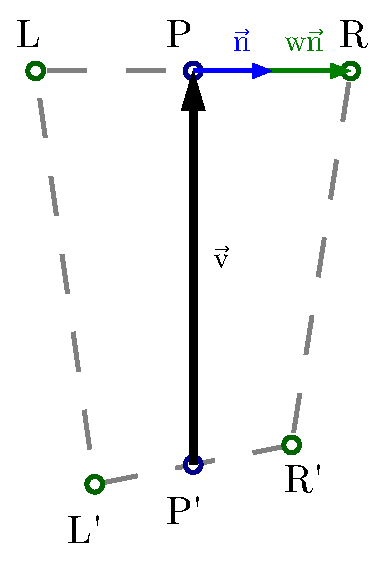
\includegraphics[height=50mm]{../img/draw-segment-quadrilateral.eps}
      \caption{Drawn quadrilateral segment of a line}
      \label{fig:draw-segment-quadrilateral}
  \end{figure}


\begin{figure}
	\centering
  		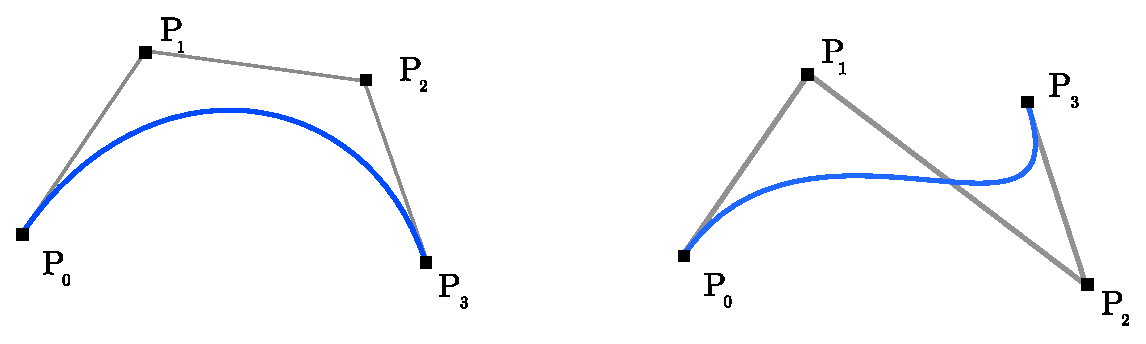
\includegraphics[width=130mm]{../img/bezier_curves.eps}
  		\caption{Bézier curve interpolation examples}
  		\label{fig:bezier-curve}
\end{figure}

The curves drawn using quadrilaterals are not very smooth. For smoother curves, straight lines must be replaced with interpolation splines. Both SVG and Canvas 2D Context implement \textit{cubic Bézier curves}. Cubic Bézier curves are defined by four control points, $ \mathbf{P}_0, \mathbf{P}_1, \mathbf{P}_2, \mathbf{P}_3 $. Path starts in $ \mathbf{P}_0 $ and ends in $ \mathbf{P}_3 $, it does not usually go through points $ \mathbf{P}_1, \mathbf{P}_2 $. The interpolation forumla of the curve is

$$ \mathbf{B}(t) = (1 - 1)^3 \mathbf{P}_0 + 3(1-t)^{2}t\mathbf{P}_1 + 3(1-t)^{2}t^2\mathbf{P}_2 + t^3\mathbf{P}_3, 0 \leq t \leq 1$$ \cite{}\footnote{An introduction to splines for use in computer graphics and geometric modeling, Bartels, Richard H, p. 160, https://cs.uwaterloo.ca/research/tr/1983/CS-83-09.pdf}

To calculate the control points of a cubic Bézier curve for segment between points $\mathbf{X}_i$ and $\mathbf{X}_{i+1}$, calculated by the DynaDraw algorithm, we can also take points $\mathbf{X}_{i-1}$ and $\mathbf{X}_{i+2}$ and look at these four points as \textit{Catmull-Rom spline} control points. Catmull-Rom is a special type of \textit{Cardinal spline}, with the tension parameter $\tau = 0$\cite{}\footnote{http://people.cs.clemson.edu/~dhouse/courses/405/notes/splines.pdf}. This approach gives us a nice smooth curve calculated just from the consequent points calcuated by the Dynadraw algorithm and also guarantee of $C^1$ continuity (@todo: citation) of the whole path.

A special conversion matrix between Catmull-Rom spline and Bézier curve is defined \cite{}\footnote{http://therndguy.com/papers/curves.pdf} and so the conversion is very straighforward. The formula for calculating cubic Bézier control points $ \mathbf{P}_0, \mathbf{P}_1, \mathbf{P}_2, \mathbf{P}_3 $, from the points $ \mathbf{X}_{i-1}, \mathbf{X}_i, \mathbf{X}_{i+1}, \mathbf{X}_{i+2} $ is

$$
\begin{pmatrix}\mathbf{P}_0 & \mathbf{P}_1 & \mathbf{P}_{2} & \mathbf{P}_{3} \end{pmatrix} = \frac{1}{6}\begin{pmatrix} 0 & 6 & 0 & 0 \\ -1 & 6 & 1 & 0 \\ 0 & 1 & 6 & -1 \\ 0 & 0 & 6 & 0 \end{pmatrix} \begin{pmatrix} \mathbf{X}_{i-1} \\ \mathbf{X}_i \\ \mathbf{X}_{i+1} \\ \mathbf{X}_{i+2} \end{pmatrix}
$$

The first and the last segments must be processed in a special way, as there is no preciding point, or following respectively. 

For an example of cubic Bézier curve, see figure~\ref{fig:bezier-curve}.



\subsubsection{Audio capturing, processing and upload}

HTML5 provides only one way to access microphone data at the moment and it is through the \textit{getUserMedia API} \cite{get_user_media}. \textit{navigator.getUserMedia} function prompts the user to for permission to use their audio input (this function is also used to access webcam stream in other applications). The \textit{navigator.getUserMedia} function is well documented on Mozilla Developer Network (MDN) \footnote{MDN: https://developer.mozilla.org/en-US/docs/Web/API/Navigator/getUserMedia} website.

If user's device has a connected microphone and user gives his permission to use his audio input, then a \textit{MediaStream} \footnote{MediaStream: http://www.w3.org/TR/mediacapture-streams/\#idl-def-MediaStream} object is provided by the browser and from this time on audio can be processed. Error callback with \textit{MediaStreamError}\footnote{MediaStreamError: http://www.w3.org/TR/mediacapture-streams/\#idl-def-MediaStreamError} instance as a parameter is called otherwise.

Current browsers implement \textit{ScriptProcessorNode} according to the W3C Working Draft from 10 October 2013 of \textit{Web Audio API}. Unfortunately, the \textit{ScriptProcessorNode} interface is deprecated in newer drafts of the specification and should be replaced with \textit{AudioWorkerNote} in the future\cite{mic_deprecated}. This new approach is not yet standardised, implemented and documented in web browsers. Both of these methods provide access to \textit{AudioBuffer} instance, which contains \tetxit{linear pulse-code modulation} (LPCM)\cite{wiki_pcm} sampled data from the microphone \cite{mic_pcm}.

This data is then sent to the server using a WebSocket. 


\subsubsection{High Resolution Timer}
To make the video look as good as possible, we need to store as precise data as possible. The \textit{Date.now()} function\footnote{https://developer.mozilla.org/en-US/docs/Web/JavaScript/Reference/Global\_Objects/Date/now} returns the number of milliseconds elapsed since 1 January 1970 00:00:00 UTC. The millisecond accuracy might seem enough, but modern browsers provide even more accurate data via the \textit{High Resolution Time} \footnote{https://dvcs.w3.org/hg/webperf/raw-file/tip/specs/HighResolutionTime/Overview.html} via the \textit{window.performance.now()} function\footnote{https://developer.mozilla.org/en-US/docs/Web/API/Performance/now} \footnote{http://updates.html5rocks.com/2012/08/When-milliseconds-are-not-enough-performance-now} with the accuracy of microseconds. The \textit{window.performance.now()} function doesn't provide data related to current time, but the milliseconds elapsed since page was loaded as a floating point number. This makes it more suitable for animation purposes.

Timing functionality is wrapped in \textit{VideoTimer} class in the Helpers module\footnote{implementation can be found in \textit{/src/VectorVideo/Helpers/VideoTimer.ts} file with a method for getting the number of milliseconds elapsed since last timer reset with the best precision provided by the web browser.



\subsubsection{Input from pointing devices}

Detecting mouse movement and the state of it's buttons is a very common task in web development. Users navigate through web pages mainly by clicking on hypertext links with their computer mouse. Therefore mouse events are well specified and work across all desktop web browsers and desktop platforms.

Unfortunately, the situation among other pointing devices other than computer mice is much less uniform. With the boom of smartphones and tablets, touchscreens are very common. Also computer graphics tablets are used by artists and many people use them when creating a Khan Academy style video.

\paragraph{Mouse input}
Event handler is passed the \textit{MouseEvent} object\footnote{http://www.w3.org/TR/DOM-Level-2-Events/events.html#Events-MouseEvent}. The relevat information are the \textit{clientX} and \textit{clientY} properties, stating current mouse posititon relative to the position of the element it is attached to. 

\paragraph{Wacom Webplugin pen API}
The Wacom Webplugin pen API (WebPAPI) is a browser plugin interface for pen data access from all Wacom consumer and professional tablets \cite{}\footnote{http://www.wacomeng.com/web/WebPluginReleaseNotes.htm}.

Unfortunatelly support for this plugin was discontinued by Chromium and Google Chrome \footnote{http://blog.chromium.org/2013/09/saying-goodbye-to-our-old-friend-npapi.htm} and therefore it should not be relied on.

\paragraph{Touch Events API}
Touch Events API is an API for handling touch input from touch screens. The standard is proposed by Apple and is implemented across many platforms and in many mobile web browsers \footnote{http://caniuse.com/\#feat=touch} \cite{}.

This API supports multiple touches at once, but this feature is not needed and neither implemented in this project. Unfortunately, this API provides no touch pressure information.

\paragraph{Pointer Events API}
Pointer Events API is an open API created by Microsoft. It's purpose is to unify the way mouse events, touch screen events, stylus and other (i.e. Kinect) similar ways into one API. This technology is implemented in Internet Explorer and will be also present in the final version of the Microsoft Edge browser. Firefox implements this API, but it is so far accessible only if a specific hidden flag is enabled. Google has announced the intent to also implement this functionality in upcoming releases of Google Chrome across all platforms.

This API also provides pressure information for pointing devices, that support this feature, including Wacom graphics tablets.



\section{Building the library}

Source code of the project can be found either among the attached files, or in git repository \textit{https://github.com/simonrozsival/vectorvideo}. Copy or clone this code to your computer.

To be able to compile the library, it is necessary to install \textit{Node.js}\footnote{https://nodejs.org/} on your computer. After installing Node.js, install all dependencies of this project by running the \verb|npm install| command in the root directory of the project's source files. You must also install \textit{Gulp} streaming build system\footnote{http://gulpjs.com} globaly by running the \verb|npm install -g gulp| command.

Build all code by running \verb|gulp| command in the same directory. This will compile all TypeScript source files into JavaScript. You can then use the compiled and minified library located in \textit{./release/vector-screencast/vector-screencast.min.js} JavaScript file. Along with the library, a web worker file \textit{./release/workers/RecordingWorker.js}, which is necessary for audio recording. Default CSS theme of the player and recorder was compiled from LESS source to \textit{./release/themes/default/theme.min.css}.

A demo audio recording server was also compiled in this process and is available in the \textit{./release/audio-server/AudioServer.js} JavaScript file. This server can used in a Node.js program.

\begin{table}
  \begin{tabular}{ll}
  \hline
  
  \verb|gulp|             &     \\ \hline 
  \verb|gulp clean|       &     \\ \hline
  \verb|gulp lib|         &     \\ \hline
  \verb|gulp demo|        & Builds the whole example project.  \\ \hline
  \verb|gulp doc|         & Generates API documentation from the TypeScript source files and comments. \\ \hline

  \end{tabular}
  \label{tbl:gulp}
  \caption{Available gulp commands}
\end{table}


For details on how to use the library in your project, see chapter~\ref{ch:integration} on page~\pageref{ch:integration}.